\documentclass[aspectratio=169,11pt]{beamer}

\usepackage[T1]{fontenc}
\usepackage{lmodern}
\usepackage{amsmath,amssymb,mathtools,booktabs,tabularx}
\usepackage{graphicx}
\usepackage{tikz}
\usetikzlibrary{arrows.meta,calc,positioning,shapes.geometric,trees}
\usepackage{tcolorbox}
\usepackage{listings}
% Beamer's \appendix bookmark uses \translate{Appendix}; expose its text to Hyperref.
\pdfstringdefDisableCommands{\def\translate#1{#1}}
\usetheme{Boadilla}
\usecolortheme{seagull}
\setbeamertemplate{navigation symbols}{}
\setbeamertemplate{items}[circle]
\setbeameroption{hide notes}
\definecolor{osblue}{RGB}{28,86,145}
\definecolor{osgreen}{RGB}{36,125,91}
\definecolor{osorange}{RGB}{202,105,36}
\definecolor{osred}{RGB}{166,45,45}
\definecolor{osgray}{RGB}{74,85,104}
\definecolor{ospurple}{RGB}{101,67,135}
\newcommand{\code}[1]{\texttt{\detokenize{#1}}}
\newcommand{\smallnote}[1]{\par\vspace{0.15em}{\scriptsize\color{osgray}#1}}
\newcolumntype{Y}{>{\raggedright\arraybackslash}X}
\lstset{
  basicstyle=\scriptsize\ttfamily,
  breaklines=true,
  showstringspaces=false,
  columns=fullflexible,
  keepspaces=true
}

% Title page information
\title[Scheduling]{Real-Time Scheduling and OS Case Studies}
\subtitle{Week 7: schedulability, fairness, and dispatching}
\author{SDB}
\date{Autumn 2026}

\begin{document}

% Title slide
\begin{frame}[plain, noframenumbering]
    \titlepage
\end{frame}

% \input{content/0-intro}
% Agenda
\begin{frame}{Agenda: Real-Time \& Modern OS Scheduling}
  \footnotesize
  \textbf{Beyond General Purpose: Predictability and Fairness in Complex Systems}
  \begin{enumerate}
    \item \textbf{Real-time models, RMS, and EDF} \hfill \textit{(schedulability and guarantees)}
    \item \textbf{Linux: CFS to EEVDF} \hfill \textit{(fairness and latency)}
    \item \textbf{Android case study} \hfill \textit{(frame timing and worker priorities)}
    \item \textbf{Windows Scheduler \& Dispatching} \hfill \textit{(responsiveness and priority management)}
    \item \textbf{macOS case study} \hfill \textit{(QoS and energy-aware work)}
    \item \textbf{Comparison \& Hands-on}
  \end{enumerate}
  \vspace{0.3cm}
  \pause
  \begin{tcolorbox}[title=\textbf{Think Ahead: When Predictability is Paramount}, colback=blue!5!white, colframe=blue!75!black, fonttitle=\bfseries]
  What assumptions make a deadline guarantee meaningful? How do fixed-priority and deadline-driven policies differ, and how do general-purpose systems trade proportional fairness against latency?
  \end{tcolorbox}
\end{frame}

% Real-time intro
\begin{frame}{Real-time scheduling: correctness includes timeliness}
  \small
  A real-time system must produce a logically correct result \emph{and} produce it before its deadline. The scheduler is only one part of that guarantee.
  \begin{itemize}
    \item \textbf{Hard:} a missed deadline is unacceptable under the stated fault model; design for bounded worst-case response.
    \item \textbf{Firm:} a late result has no value, but occasional misses may be tolerated.
    \item \textbf{Soft:} late results retain value; quality or utility degrades with lateness.
  \end{itemize}
  \begin{tcolorbox}[title=Guarantee boundary,colback=orange!5,colframe=orange!70]
    A schedulability proof is conditional on a workload model, WCET bounds, release jitter, blocking, interrupt and dispatch costs, platform behavior, and the assumed fault model. A scheduler name alone is not a guarantee.
  \end{tcolorbox}
  \note{Emphasize that hard real-time is not synonymous with "fast." It is a claim about a bounded response under explicitly stated assumptions. A WCET estimate must include relevant cache, memory, I/O, interrupt, and synchronization effects.}
\end{frame}

\begin{frame}{Periodic task model and timing vocabulary}
  \small
  \begin{columns}[T,onlytextwidth]
    \column{0.52\textwidth}
      \begin{itemize}
        \item $T_i$: minimum inter-arrival time / period of task $\tau_i$.
        \item $C_i$: worst-case execution demand of one job.
        \item $D_i$: relative deadline; absolute deadline is release time plus $D_i$.
        \item $J_i$: release jitter; $B_i$: maximum blocking from lower-priority work.
        \item $R_i$: worst-case response time from release to completion.
      \end{itemize}
      Utilization for implicit-deadline periodic tasks is $U=\sum_i C_i/T_i$.
    \column{0.44\textwidth}
      \centering
      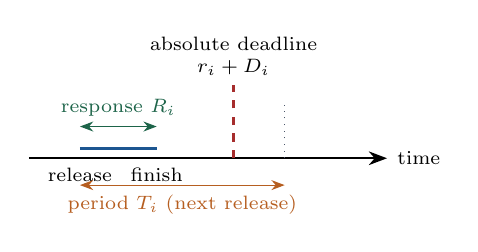
\begin{tikzpicture}[x=.65cm,y=.62cm,font=\scriptsize,>=Stealth]
        \draw[->,thick] (0,0)--(7,0) node[right]{time};
        \draw[osblue,very thick] (1,.2)--(2.5,.2);
        \node[below] at (1,0) {release};
        \node[below] at (2.5,0) {finish};
        \draw[osred,dashed,thick] (4,0)--(4,1.5);
        \node[above,align=center] at (4,1.5) {absolute deadline\\$r_i+D_i$};
        \draw[<->,osgreen!80!black] (1,.65)--(2.5,.65)
          node[midway,above]{response $R_i$};
        \draw[<->,osorange!90!black] (1,-.55)--(5,-.55)
          node[midway,below]{period $T_i$ (next release)};
        \draw[osgray,dotted] (5,0)--(5,1.1);
      \end{tikzpicture}
  \end{columns}
  \smallnote{Basic uniprocessor results below assume independent, preemptible jobs, bounded execution, and negligible overhead unless a slide says otherwise.}
\end{frame}

% RMS
\begin{frame}{Rate-monotonic scheduling: fixed-priority optimality}
  \scriptsize
  \begin{block}{Priority assignment}
    For periodic tasks with $D_i=T_i$, assign higher fixed priority to shorter periods:
    \[
      T_i<T_j \quad\Longrightarrow\quad \tau_i\text{ has higher priority than }\tau_j.
    \]
  \end{block}
  \textbf{Classical model:}
  \begin{itemize}
    \item single preemptive processor; independent periodic or sporadic tasks;
    \item known WCET $C_i$, implicit deadlines $D_i=T_i$, no self-suspension;
    \item no blocking or overhead in the elementary utilization theorem.
  \end{itemize}
  \textbf{Liu--Layland sufficient utilization bound:}
  \[
    U=\sum_{i=1}^{n}\frac{C_i}{T_i}\leq n\bigl(2^{1/n}-1\bigr).
  \]
  \begin{alertblock}{Interpretation}
    Passing certifies schedulability in this model. Failing this sufficient bound is \emph{inconclusive}, not proof of a missed deadline. As $n\to\infty$, the bound tends to $\ln 2\approx0.693$.
  \end{alertblock}
  \smallnote{For constrained deadlines $D_i\leq T_i$, shorter relative deadline gives higher priority under Deadline Monotonic (DM); do not automatically apply RMS ordering when $D_i\ne T_i$.}
  \note{The optimality statement is precise: rate-monotonic assignment is optimal among fixed-priority assignments for the classical independent periodic, implicit-deadline, preemptive uniprocessor model. It is not an optimality claim for multiprocessors or arbitrary deadlines.}
\end{frame}

\begin{frame}{Fixed-priority analysis: response-time recurrence}
  \small
  When utilization tests are inconclusive, compute each task's worst-case response time in priority order. In the basic model:
  \[
    R_i^{(k+1)}=C_i+\sum_{j\in hp(i)}
      \left\lceil\frac{R_i^{(k)}}{T_j}\right\rceil C_j,
    \qquad R_i^{(0)}=C_i.
  \]
  A task is schedulable if the recurrence converges to $R_i\leq D_i$ for every task. With blocking or jitter, the recurrence must include the corresponding terms.
  \begin{exampleblock}{A set the utilization bound does not certify}
    $\tau_1=(C_1,T_1)=(1,2)$ and $\tau_2=(1,3)$ give $U=5/6\approx0.833$, just above the $n=2$ bound $0.828$. For $\tau_2$, iteration gives $1\to2\to2$, so $R_2=2\leq3$; both tasks meet deadlines in this model.
  \end{exampleblock}
  \note{The recurrence counts the maximum number of higher-priority jobs that can interfere in a response window. This is exact for the stated fixed-priority model; add blocking $B_i$ and release jitter terms for more realistic systems.}
\end{frame}

% RMS Example
\begin{frame}{RMS example: utilization test and schedule}
  \small
  \begin{columns}[T,onlytextwidth]
    \column{0.43\textwidth}
      \textbf{Implicit-deadline tasks}
      \[
        (C_1,T_1)=(1,4),\qquad(C_2,T_2)=(2,6).
      \]

      Shorter-period task $\tau_1$ has higher fixed priority.
      \[
        U=\frac14+\frac26=0.583.
      \]
      \[
        U_{LL}(2)=2(\sqrt2-1)\approx0.828.
      \]
      Since $U\leq U_{LL}$, the sufficient test certifies schedulability under the classical assumptions.
    \column{0.54\textwidth}
      \centering
      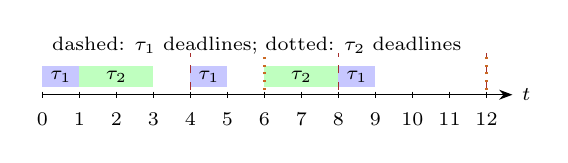
\begin{tikzpicture}[x=.47cm,y=.5cm,font=\scriptsize,>=Stealth]
        \draw[->] (0,0)--(12.7,0) node[right]{$t$};
        \foreach \x in {0,...,12} \draw (\x,.08)--(\x,-.08) node[below=2pt]{\x};
        \fill[blue!22] (0,.2) rectangle (1,.72); \node at (.5,.46){$\tau_1$};
        \fill[green!25] (1,.2) rectangle (3,.72); \node at (2,.46){$\tau_2$};
        \fill[blue!22] (4,.2) rectangle (5,.72); \node at (4.5,.46){$\tau_1$};
        \fill[green!25] (6,.2) rectangle (8,.72); \node at (7,.46){$\tau_2$};
        \fill[blue!22] (8,.2) rectangle (9,.72); \node at (8.5,.46){$\tau_1$};
        \foreach \x in {4,8,12} \draw[osred,dashed] (\x,.12)--(\x,1.05);
        \foreach \x in {6,12} \draw[osorange,dotted,thick] (\x,.12)--(\x,1.05);
        \node[anchor=west] at (0,1.25) {dashed: $\tau_1$ deadlines; dotted: $\tau_2$ deadlines};
      \end{tikzpicture}
  \end{columns}
  \smallnote{The schedule is illustrative; the utilization bound, not this finite trace, is the guarantee.}
  \note{The first job of $\tau_2$ waits for $\tau_1$ at t=0 and then runs from 1 to 3. At t=6 the next $\tau_2$ job runs until t=8; the next $\tau_1$ job is released at t=8. This one release pattern meets all shown deadlines.}
\end{frame}

% EDF
\begin{frame}{Earliest-deadline-first scheduling}
  \small
  At each scheduling decision, run the ready job with the earliest \textbf{absolute deadline}. A newly released job may preempt the running job when its deadline is earlier.
  \begin{block}{Exact utilization test: a special case}
    On one preemptive processor, for independent periodic/sporadic tasks with known WCET, no overhead or blocking, and \textbf{implicit deadlines} $D_i=T_i$:
    \[
      \sum_i\frac{C_i}{T_i}\leq1
      \quad\Longleftrightarrow\quad \text{EDF is schedulable.}
    \]
  \end{block}
  \begin{itemize}
    \item This is a necessary-and-sufficient utilization test only for that implicit-deadline model.
    \item Under overload, EDF can miss deadlines; the miss pattern depends on the arrivals and workload.
    \item For other deadline models, use demand-based analysis rather than treating $U\leq1$ as sufficient.
  \end{itemize}
  \note{EDF's optimality and utilization result are uniprocessor statements. Do not transfer the 100\% test to constrained-deadline tasks, multiprocessors, or systems with unmodeled overhead.}
\end{frame}

\begin{frame}{EDF with constrained deadlines: demand-bound test}
  \small
  For periodic or sporadic tasks with $D_i\leq T_i$, a job-demand view captures deadline density:
  \[
    \operatorname{dbf}_i(t)=
      \max\!\left(0,\left\lfloor\frac{t-D_i}{T_i}\right\rfloor+1\right)C_i.
  \]
  In the ideal preemptive uniprocessor model, EDF is feasible iff for every interval length $t>0$:
  \[
    \sum_i \operatorname{dbf}_i(t)\leq t.
  \]
  \begin{tcolorbox}[title=Why utilization alone can fail,colback=orange!5,colframe=orange!70]
    A short relative deadline can concentrate execution demand early even when average utilization $\sum_i C_i/T_i$ is below one. The demand-bound function asks whether any interval contains more work due than the processor can execute.
  \end{tcolorbox}
  \note{Define dbf as the maximum execution demand of jobs both released and due within an interval of length t. The all-interval condition is exact for constrained-deadline sporadic task systems on one preemptive processor; real implementations add overhead and blocking terms.}
\end{frame}

% EDF example
\begin{frame}{EDF example: deadline order and idle intervals}
    \small
    \textbf{Implicit-deadline tasks:} $\tau_1=(C_1,T_1)=(1,4)$ and $\tau_2=(C_2,T_2)=(2,6)$.
    \[
      U=\frac14+\frac26=\frac{7}{12}\approx0.583<1.
    \]
    Both tasks are schedulable by the implicit-deadline EDF theorem under the stated ideal model.
    \begin{center}
        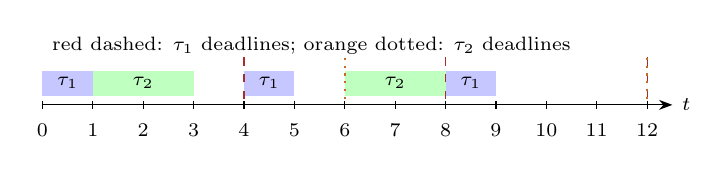
\begin{tikzpicture}[x=.64cm,y=.58cm,font=\scriptsize,>=Stealth]
            \draw[->] (0,0)--(12.5,0) node[right]{$t$};
            \foreach \x in {0,...,12} \draw (\x,.08)--(\x,-.08) node[below=2pt]{\x};
            \fill[blue!22] (0,.2) rectangle (1,.75); \node at (.5,.475) {$\tau_1$};
            \fill[green!25] (1,.2) rectangle (3,.75); \node at (2,.475) {$\tau_2$};
            \fill[blue!22] (4,.2) rectangle (5,.75); \node at (4.5,.475) {$\tau_1$};
            \fill[green!25] (6,.2) rectangle (8,.75); \node at (7,.475) {$\tau_2$};
            \fill[blue!22] (8,.2) rectangle (9,.75); \node at (8.5,.475) {$\tau_1$};
            \foreach \x in {4,8,12} \draw[osred,dashed] (\x,.13)--(\x,1.05);
            \foreach \x in {6,12} \draw[osorange,dotted,thick] (\x,.13)--(\x,1.05);
            \node[anchor=west,align=left] at (0,1.3)
              {red dashed: $\tau_1$ deadlines; orange dotted: $\tau_2$ deadlines};
        \end{tikzpicture}
    \end{center}
    \smallnote{The chart is one valid schedule; it is not the schedulability proof. At equal absolute deadlines, either tie-break is valid here.}
    \note{Releases occur at multiples of each period; relative deadlines equal periods. The processor is idle in [3,4), [5,6), and [9,12). Separate the utilization theorem from a finite-horizon schedule drawing.}
\end{frame}

% Legacy derivation retained below only as source-history marker
\iffalse
\begin{frame}[allowframebreaks]{Earliest Deadline First (EDF): Dynamic Priority for Real-Time}
  \small
  \textbf{Concept:}
  \begin{itemize}
    \item \textbf{Dynamic Priority:} Priorities are re-calculated at each scheduling point (arrival, completion, preemption).
    \item The process with the \textbf{earliest absolute deadline} (arrival time + relative deadline) runs first.
    \item If two tasks have the same deadline, FCFS is typically used as a tie-breaker.
  \end{itemize}

  \vspace{0.3cm}
  \textbf{Assumptions for Basic EDF:}
  \begin{itemize}
    \item Tasks are periodic or aperiodic with known execution times and deadlines.
    \item Deadlines are usually equal to or less than the period.
    \item Context switch time is negligible.
  \end{itemize}

  \framebreak
  
  \vspace{0.3cm}
  \textbf{Schedulability Test:}
  For a set of $n$ independent periodic tasks, EDF can guarantee schedulability if their total CPU utilization $U$ is:
  \[
  U = \sum_{i=1}^{n} \frac{C_i}{T_i} \leq 1
  \]
  \textit{EDF is considered \textbf{optimal} because it can fully utilize the CPU (up to 100\%) if the tasks are schedulable.}

  \vspace{0.3cm}
  \textbf{Pros \& Cons:}
  \begin{itemize}
    \item \textbf{\textcolor{green!50!black}{Pros:}} Higher CPU utilization (up to 100\% if schedulable), more flexible than RMS, can handle aperiodic tasks well.
    \item \textbf{\textcolor{red!70!black}{Cons:}} More complex to implement due to dynamic priorities, higher runtime overhead (recalculating priorities), unpredictable behavior if overloaded (all tasks might miss deadlines).
  \end{itemize}
\end{frame}
\fi

% Previous EDF schedule is superseded by the annotated example above.
\iffalse
\begin{frame}{EDF Example: Dynamic Priorities in Action}
    \small
    \textbf{Tasks:} (Execution Time $C_i$, Period $T_i$, Deadline $D_i$ (=$T_i$))
    \begin{itemize}
        \item Task 1 (P1): $C_1=1$, $T_1=4$
        \item Task 2 (P2): $C_2=2$, $T_2=6$
    \end{itemize}
    \pause
    \textbf{Step 1: Calculate Utilization ($U$)}
    \[
    U = \frac{C_1}{T_1} + \frac{C_2}{T_2} = \frac{1}{4} + \frac{2}{6} = 0.25 + 0.333 = \textbf{0.583}
    \]
    \pause
    \textbf{Step 2: Apply EDF Schedulability Test}
    $U = 0.583 \leq 1$. The task set is \textbf{schedulable by EDF}.
    \vspace{0.3cm}
    \pause
    
    \textbf{Step 3: Corrected Execution (Gantt Chart)}
    \textit{(Tasks arrive at $t=0$, $4$, $6$, $8$, etc. Deadlines are $T_i$ from arrival.)}
    \begin{center}
        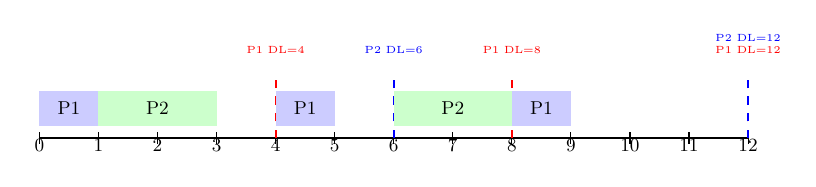
\begin{tikzpicture}[scale=0.75, transform shape, font=\small]
            % Time axis
            \draw[thick] (0,0) -- (12,0);
            \foreach \x in {0,1,2,3,4,5,6,7,8,9,10,11,12}
                \draw (\x, -0.1) -- (\x, 0.1) node[below] {\x};

            % Deadlines (DLs)
            % P1 instances: t=0 (DL 4), t=4 (DL 8), t=8 (DL 12)
            \draw[red, dashed, thick] (4, 0) -- (4, 1.0) node[above=0.3cm, font=\tiny, align=center] {P1 DL=4};
            \draw[red, dashed, thick] (8, 0) -- (8, 1.0) node[above=0.3cm, font=\tiny, align=center] {P1 DL=8};
            \draw[red, dashed, thick] (12, 0) -- (12, 1.0) node[above=0.3cm, font=\tiny, align=center] {P1 DL=12};

            % P2 instances: t=0 (DL 6), t=6 (DL 12)
            \draw[blue, dashed, thick] (6, 0) -- (6, 1.0) node[above=0.3cm, font=\tiny, align=center] {P2 DL=6};
            \draw[blue, dashed, thick] (12, 0) -- (12, 1.0) node[above=0.3cm, font=\tiny, align=center] [yshift=2mm]{P2 DL=12};

            % Correct EDF Execution Blocks
            % T=0: P1 (DL=4) vs P2 (DL=6). P1 wins. P1 runs for its full 1 unit.
            \fill[blue!20] (0,0.2) rectangle (1,0.8); \node at (0.5,0.5) {P1};
            % T=1: P1 finished. P2 is only ready task. P2 runs for its full 2 units.
            \fill[green!20] (1,0.2) rectangle (3,0.8); \node at (2,0.5) {P2};
            % T=3-4: Both tasks complete for this period. CPU is Idle.
            % T=4: New P1 instance (DL=8). P2's next instance is at t=6. P1 is the only ready task. P1 runs for its full 1 unit.
            \fill[blue!20] (4,0.2) rectangle (5,0.8); \node at (4.5,0.5) {P1};
            % T=5-6: P1 is done. P2's next instance has not arrived yet. CPU is Idle.
            % T=6: New P2 instance (DL=12). P1's next instance is at t=8. P2 has earliest deadline (12 vs 16 for P1's new). P2 runs for its full 2 units.
            \fill[green!20] (6,0.2) rectangle (8,0.8); \node at (7,0.5) {P2};
            % T=8: New P1 instance (DL=12). P1 and P2 have same deadline. Common tie-break is to run lower ID task. P1 runs for its full 1 unit.
            \fill[blue!20] (8,0.2) rectangle (9,0.8); \node at (8.5,0.5) {P1};
            % T=9-12: P1 is done, P2 is done. CPU is Idle until t=12.
        \end{tikzpicture}
    \end{center}
    \vspace{0.1cm}
    \textit{All deadlines are met by dynamically scheduling the task with the earliest deadline.}
\end{frame}
\fi

% RMS vs EDF
\begin{frame}{RMS vs EDF: A Direct Comparison}
  \scriptsize
  \begin{tabularx}{\textwidth}{@{}lYY@{}}
  \toprule
  \textbf{Property} & \textbf{Rate monotonic (fixed priority)} & \textbf{EDF (dynamic priority)} \\
  \midrule
  Priority key & Shorter period gets higher fixed priority & Earlier absolute deadline gets higher priority \\
  Classical exact/sufficient test & Response-time analysis; LL utilization bound is sufficient only & $U\leq1$ iff feasible for implicit deadlines; DBF for constrained deadlines \\
  Overload & Fixed priority is stable/predictable by priority, but low-priority jobs can miss & Earliest-deadline order is optimal in the ideal uniprocessor model; overload still causes misses \\
  Practical caveat & Blocking, jitter, and execution overhead must be modeled & Same; multiprocessor guarantees differ from uniprocessor results \\
  \bottomrule
  \end{tabularx}
  \smallnote{Both rows compare idealized preemptive uniprocessor models; neither method makes WCET or blocking disappear.}
\end{frame}

% The following historical CFS/Windows exposition is retained only as source
% history; its visible replacements immediately follow the block.
\iffalse
% Linux CFS
\begin{frame}[allowframebreaks]{Linux CFS (Completely Fair Scheduler): General Purpose Fairness}
  \small
  \textbf{Concept:} Introduced in Linux kernel 2.6.23, CFS is the default scheduler for normal (non-real-time) processes. Its primary goal is \textbf{fairness} – ensuring that all processes receive a "fair" share of CPU time relative to their assigned weight.
  \vspace{0.3cm}
  \textbf{Key Principles:}
  \begin{itemize}
    \item \textbf{Proportional Share:} Instead of fixed time slices (like Round Robin), CFS aims for a proportional distribution of CPU time based on task "weight".
    \item \textbf{Virtual Runtime (vruntime):} Each runnable task has a `vruntime' value, which tracks the amount of time it would have run on an "ideal" perfectly fair CPU.
    \item \textbf{Red-Black Tree:} The runnable tasks are stored in a red-black tree, sorted by their `vruntime'. The task with the smallest `vruntime' (meaning it's "fallen behind" the most in terms of CPU allocation) is always picked next.
    \item \textbf{Minimizing Latency:} While fairness is primary, CFS also tries to keep interactive task latency low.
  \end{itemize}

  \textbf{\textcolor{green!50!black}{Pros:}}
    \begin{itemize}
    \item \textbf{Excellent Fairness:} The scheduler tracks the virtual runtime of each process, ensuring every process gets a "fair" share of CPU time over time. No single process can dominate the CPU.
    \item \textbf{Highly Scalable:} It uses efficient data structures (like a red-black tree) to manage processes, allowing it to scale effectively with a large number of cores and thousands of processes without performance bottlenecks.
    \item \textbf{Good Responsiveness for Interactive Tasks:} Processes that spend more time waiting for user input get a higher priority when they are ready to run again. This makes the system feel quick and responsive.
    \item \textbf{No Starvation:} Every process is guaranteed to eventually run. As a process waits, its priority effectively increases until it is chosen by the scheduler, eliminating the risk of waiting indefinitely.
\end{itemize}

\vspace{0.5cm}
\textbf{\textcolor{red!70!black}{Cons:}}
\begin{itemize}
    \item \textbf{Not Suitable for Hard Real-Time Tasks:} These schedulers prioritize fairness over strict deadlines. They cannot guarantee that a critical task will be executed by a specific time, making them unsuitable for mission-critical real-time systems.
    \item \textbf{Higher Overhead than Simpler Schedulers:} To achieve their goals, these schedulers use more complex logic and data structures. This results in a slightly higher overhead compared to very simple schedulers like First-Come, First-Served (FCFS) or Round-Robin (RR).
\end{itemize}
\end{frame}

% CFS Visualization
\begin{frame}{CFS: The Run Queue as a Red-Black Tree}
\small
\textbf{Concept:} The red-black tree in CFS acts as the ``run queue". It's a self-balancing binary search tree that keeps tasks sorted by their `vruntime'.

% \vspace{0.3cm}
\textbf{Illustration:}

\centering
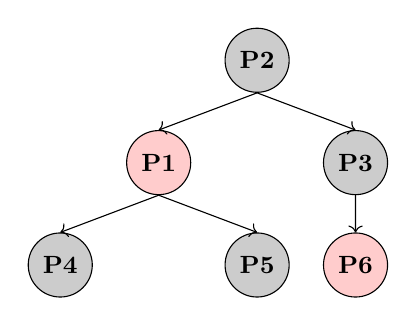
\begin{tikzpicture}[
    every node/.style={circle,draw,minimum size=.4cm, font=\small\bfseries},
    level distance=1.3cm,
    sibling distance=2.5cm,
    edge from parent/.style={draw,->},
    edge from parent path={(\tikzparentnode.south) -- (\tikzchildnode.north)}
]
    \node[fill=black!20] (p2) {P2}
    child { node[fill=red!20] (p1) {P1}
        child { node[fill=black!20] (p4) {P4}}
        child { node[fill=black!20] (p5) {P5}}
    }
    child { node[fill=black!20] (p3) {P3}
        child { node[fill=red!20] (p6) {P6}}
    };
    
\end{tikzpicture}

\vspace{0.5cm}
\textbf{How it works:}

\begin{itemize}
    \item The process with the smallest `vruntime' is always the leftmost node (e.g., P1). It gets chosen to run.
    \item When a process's time slice expires, its `vruntime' is updated.
    \item The process is then \textbf{re-inserted} into a new position in the tree, based on its new `vruntime' value.
\end{itemize}
\end{frame}

% CFS logic
\begin{frame}[allowframebreaks]{Linux CFS: The vruntime Calculation}
  \small
  \textbf{Goal:} Ensure processes get CPU time proportional to their "weight" (derived from `nice' value).

  \vspace{0.3cm}
  \textbf{Simplified vruntime Formula (Conceptual):}
  \[
  \text{vruntime}_{\text{new}} = \text{vruntime}_{\text{old}} + \left( \text{actual\_CPU\_run\_time} \times \frac{\text{SCHED\_NICE\_WEIGHT\_HZ}}{\text{task\_weight}} \right)
  \]
  \vspace{0.3cm}
  \textbf{Key Components:}
  \begin{itemize}
    \item \textbf{`actual\_CPU\_run\_time':} The real CPU time the task just consumed.
    \item \textbf{`nice\_value' (User-set priority):}
      \begin{itemize}
        \item A user-set value (from -20 to +19, default 0).
        \item Lower `nice' value (e.g., -20) implies higher user preference.
      \end{itemize}
\framebreak
    \item \textbf{`task\_weight' (Derived from `nice\_value'):}
      \begin{itemize}
        \item A lookup table maps `nice\_value' to `task\_weight'.
        \item Higher `task\_weight' means the task deserves more CPU time (and its `vruntime' will increase slower for the same actual runtime).
        \item Example: `nice 0' has a weight of 1024. `nice 1' has weight 820. `nice -5' has weight 2379.
      \end{itemize}
    \item \textbf{`SCHED\_NICE\_WEIGHT\_HZ':} A constant for normalization (1024 in many kernels, corresponding to nice 0's weight).
  \end{itemize}
  \vspace{0.1cm}
  \textit{Essentially, `vruntime' aims to track normalized CPU usage. A task with a lower `nice' value (higher weight) will see its `vruntime' increase slower, meaning it stays closer to the leftmost part of the red-black tree and gets scheduled more often.}
\end{frame}

% Windows Scheduler
\begin{frame}[allowframebreaks]{Windows Scheduling Mechanism: Priority-Based Responsiveness}
  \small
  \textbf{Overview:} The Windows scheduler (Dispatcher) is a priority-based, preemptive, and multi-level feedback queue scheduler that operates on threads.
  \vspace{0.3cm}
  \textbf{Key Features:}
  \begin{itemize}
    \item \textbf{32 Priority Levels:}
      \begin{itemize}
        \item \textbf{Real-Time (16-31):} Fixed priorities, for system-critical tasks. No dynamic changes.
        \item \textbf{Dynamic (1-15):} Priorities can change based on system activity (aging, boosting).
        \item \textbf{Zero (0):} Special system idle thread.
      \end{itemize}
\framebreak
    \item \textbf{Dynamic Priority Adjustments:}
      \begin{itemize}
        \item \textbf{Boosting:} Threads receive temporary priority boosts for various reasons (e.g., completing I/O, becoming foreground application, user input). This enhances responsiveness.
        \item \textbf{Decaying (Aging):} After a quantum expires or a boost expires, a thread's dynamic priority is typically lowered (decayed) over time, unless it's a critical thread.
      \end{itemize}
    \item \textbf{Quantum-Based Preemption:} Each thread runs for a fixed time quantum. When the quantum expires, the thread is preempted.
    \item \textbf{Dispatcher Object:} The central component that selects the highest-priority runnable thread and performs context switching.
  \end{itemize}
\framebreak
  \vspace{0.3cm}
  \textbf{Emphasis:} Windows scheduling strongly emphasizes \textbf{responsiveness for interactive applications} (especially foreground UI threads) through its boosting and priority management mechanisms.
  \vspace{0.3cm}
  \textbf{Pros \& Cons:}
  \begin{itemize}
    \item \textbf{\textcolor{green!50!black}{Pros:}} Excellent responsiveness for interactive tasks, good balance between throughput and latency, robust priority management.
    \item \textbf{\textcolor{red!70!black}{Cons:}} Can be complex to predict exact behavior, potential for priority inversion (though mitigations exist), not designed for hard real-time guarantees.
  \end{itemize}
\end{frame}

% Comparative Slide
\begin{frame}{Comparing Linux CFS and Windows Scheduler}
  \small
  \resizebox{\textwidth}{!}
  {
  \begin{tabular}{|l|c|c|}
  \hline
  \textbf{Feature} & \textbf{Linux CFS} & \textbf{Windows Scheduler} \\
  \hline
  \textbf{Core Philosophy} & Proportional Share / Fairness & Priority-based / Responsiveness \\
  \textbf{Preemption} & Yes (based on `vruntime' / quantum) & Yes (based on priority / quantum) \\
  \textbf{Priority Management} & Dynamic `vruntime' (from `nice' value) & 32 fixed + dynamic levels (boosting/decaying) \\
  \textbf{Run Queue Structure} & Red-Black Tree & Ready queues (one per priority level) \\
  \textbf{Starvation Prevention} & Inherent in `vruntime' fairness model & Aging and Priority Boosting \\
  \textbf{Real-Time Support} & Separate `SCHED\_FIFO'/`SCHED\_RR' policies & Dedicated Real-Time priority levels (16-31) \\
  \textbf{Typical Workload} & Servers, Desktops, Embedded (fair for all types) & Desktops, Workstations (optimized for interactivity) \\
  \hline
  \end{tabular}
  }
\end{frame}

\fi

\begin{frame}{Linux scheduling classes: policy is not one algorithm}
  \small
  Linux schedules runnable \textbf{threads/tasks}, not abstract processes. The kernel organizes scheduling policies into classes; higher-class runnable work can preempt lower-class work.
  \begin{center}
    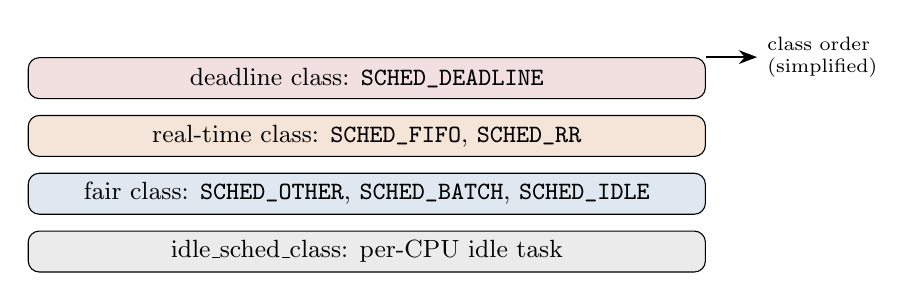
\begin{tikzpicture}[node distance=2mm,font=\small,>=Stealth,
      cl/.style={draw,rounded corners,minimum width=8.6cm,minimum height=.52cm,align=center}]
      \node[cl,fill=osred!15] (dl) {deadline class: \code{SCHED_DEADLINE}};
      \node[cl,fill=osorange!18,below=of dl] (rt) {real-time class: \code{SCHED_FIFO}, \code{SCHED_RR}};
      \node[cl,fill=osblue!14,below=of rt] (fair) {fair class: \code{SCHED_OTHER}, \code{SCHED_BATCH}, \code{SCHED_IDLE}};
      \node[cl,fill=black!8,below=of fair] (idle) {idle\_sched\_class: per-CPU idle task};
      \draw[-{Stealth},thick] (dl.north east)--++(.65,0) node[right,align=left,font=\scriptsize]{class order\\(simplified)};
    \end{tikzpicture}
  \end{center}
  \begin{itemize}
    \item \code{nice} adjusts fair-class weight; \code{SCHED_IDLE} is a fair policy, distinct from the CPU idle-task class.
    \item Run queues are per-CPU; affinity, migration, load balancing, and CPU topology affect observed behavior.
    \item The normal fair class targets proportional sharing and latency—not hard-deadline certification.
  \end{itemize}
  \smallnote{Class names and internals are Linux implementation details; consult documentation for the target kernel version.}
  \note{The diagram omits stop-task and implementation-specific details, and should be read as a simplified class hierarchy. A real-time or deadline task can dominate fair-class work, subject to kernel policy and limits.}
\end{frame}

\begin{frame}{Linux fair scheduling: from CFS to EEVDF}
  \scriptsize
  \begin{columns}[T,onlytextwidth]
    \column{0.49\textwidth}
      \begin{block}{CFS: useful historical model}
        Track normalized service as virtual runtime. Conceptually, the runnable entity with the smallest virtual runtime is most under-served and becomes eligible to run.
      \end{block}
      \begin{itemize}
        \item Run-queue ordering historically used a red-black tree.
        \item This remains useful for understanding weight-based proportional fairness.
      \end{itemize}
    \column{0.47\textwidth}
      \begin{block}{EEVDF: modern fair-scheduler direction}
        Lag represents weighted ideal service minus actual service: positive lag means an entity is owed CPU. Select the earliest virtual deadline among eligible entities (nonnegative lag).
      \end{block}
      \begin{itemize}
        \item A virtual deadline is an ordering key, not the application's real-time deadline.
        \item Requested slice length participates in virtual-deadline ordering, exposing latency/throughput trade-offs.
      \end{itemize}
  \end{columns}
  \begin{tcolorbox}[title=Interpretation,colback=orange!5,colframe=orange!70]
    Do not teach “the current Linux scheduler always picks the leftmost $v_{runtime}$ node” as a version-independent fact. CFS is the conceptual predecessor; current mainline fair scheduling uses EEVDF mechanisms, and deployed kernels can differ by version/configuration.
  \end{tcolorbox}
  \note{Linux began transitioning its fair scheduler to EEVDF in the 6.6 era. EEVDF's eligibility/virtual-deadline view preserves weighted fairness while better representing requested latency. Point students to the official scheduler documentation for exact version-specific internals.}
\end{frame}

\begin{frame}{Fair-class accounting: why weights matter}
  \small
  A simplified CFS-style accounting relation is
  \[
    \Delta v_i \approx \Delta t_i\frac{W_0}{w_i},
    \qquad W_0=1024\text{ (nice-0 reference weight)}.
  \]
  Larger weight $w_i$ means virtual service grows more slowly for the same execution time, so the entity receives a larger long-run share.
  \begin{center}
    \begin{tabular}{lrr}
      \toprule
      Runnable task & Relative weight & Idealized share of two-task CPU \\
      \midrule
      nice 0 & 1024 & $1024/(1024+335)\approx75.3\%$ \\
      nice +5 & 335 & $335/(1024+335)\approx24.7\%$ \\
      \bottomrule
    \end{tabular}
  \end{center}
  \begin{itemize}
    \item Shares are approximate long-run proportions among runnable peers on the same fair run queue.
    \item Sleep, cgroup hierarchy, CPU affinity, quota, competing classes, and multicore placement change the realized share.
  \end{itemize}
  \note{The weight table is kernel-defined; nice levels are logarithmic, not additive percentages. The equation is an explanatory approximation, not a stable kernel ABI.}
\end{frame}

\begin{frame}{Real-time policies in Linux: reservation versus priority}
  \scriptsize
  \begin{tabularx}{\textwidth}{@{}lYY@{}}
    \toprule
    Policy & Dispatch rule (simplified) & Main risk / use \\
    \midrule
    \code{SCHED_FIFO} & Fixed RT priority; run until block, yield, or preempted by higher priority & Starvation if a high-priority thread fails to block \\
    \code{SCHED_RR} & FIFO among same-priority threads with a time quantum & Quantum is not a deadline guarantee \\
    \code{SCHED_DEADLINE} & EDF-like deadlines with Constant Bandwidth Server reservation & Admission control and runtime/period constraints required \\
    \bottomrule
  \end{tabularx}
  \begin{itemize}
    \item Deadline scheduling parameters are commonly described as runtime $Q$, relative deadline $D$, and period $T$.
    \item A reservation limits interference from a task; it does not bound device, firmware, interrupt, or application WCET by itself.
    \item Privilege, resource limits, kernel configuration, and admission control govern whether a request is accepted.
  \end{itemize}
  \begin{alertblock}{Engineering rule}
    Never run an unbounded busy loop at elevated real-time priority on a production system.
  \end{alertblock}
  \note{Linux SCHED_DEADLINE combines GEDF selection with CBS-style bandwidth enforcement. Its admission test is part of the OS resource model, not a certification that an arbitrary application meets a hard deadline end-to-end.}
\end{frame}

\begin{frame}{Why uniprocessor schedulability does not transfer to multicore}
  \small
  \begin{columns}[T,onlytextwidth]
    \column{0.48\textwidth}
      \begin{block}{Partitioned scheduling}
        Assign each task to one CPU; schedule locally.
      \end{block}
      \begin{itemize}
        \item Simple affinity and local analysis.
        \item Bin-packing can leave unusable capacity on one core while another is overloaded.
      \end{itemize}
    \column{0.48\textwidth}
      \begin{block}{Global scheduling}
        One shared ready set; migrate jobs among CPUs.
      \end{block}
      \begin{itemize}
        \item Can improve load balance.
        \item Migration, cache warmth, contention, and global analysis complicate bounds.
      \end{itemize}
  \end{columns}
  \begin{center}
    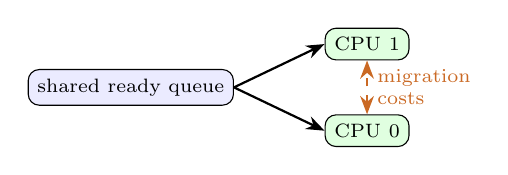
\begin{tikzpicture}[font=\scriptsize,>=Stealth]
      \node[draw,rounded corners,fill=blue!8,minimum width=2.1cm] (q) at (0,0) {shared ready queue};
      \node[draw,rounded corners,fill=green!12] (c0) at (3,-.55) {CPU 0};
      \node[draw,rounded corners,fill=green!12] (c1) at (3,.55) {CPU 1};
      \draw[->,thick] (q.east)--(c0.west);
      \draw[->,thick] (q.east)--(c1.west);
      \draw[<->,dashed,osorange,thick] (c0.north)--(c1.south)
        node[midway,right,align=left]{migration\\costs};
    \end{tikzpicture}
  \end{center}
  \smallnote{Global EDF and partitioned EDF have different feasibility properties; $U\leq m$ is not a universal multiprocessor feasibility test.}
\end{frame}

\begin{frame}{Case study: Android frame timing and background work}
  \scriptsize
  \begin{columns}[T,onlytextwidth]
    \column{0.49\textwidth}
      \begin{itemize}
        \item At 60 Hz, a refresh is about $16.7$ ms. App work must finish early enough for rendering and composition; this is a budget, not a reserved CPU slice.
        \item Keep input and frame-state updates short on the UI thread. Move decoding and I/O to bounded workers.
        \item Use \code{Process.setThreadPriority} conservatively; background priority suits deferrable worker work.
        \item Excessive priority can contend with UI/RenderThread and increase dropped frames. More threads do not create CPU capacity.
      \end{itemize}
      \begin{tcolorbox}[title=What the case teaches,colback=osorange!5,colframe=osorange!70]
        Frame timing is end-to-end: app, GPU, compositor, and device load all matter. Priority is not a frame-deadline reservation.
      \end{tcolorbox}
    \column{0.49\textwidth}
      \centering
      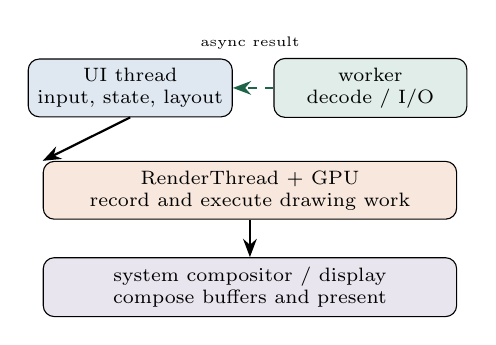
\begin{tikzpicture}[font=\scriptsize,>=Stealth,
        app/.style={draw,rounded corners,align=center,minimum height=.68cm,minimum width=2.45cm},
        stage/.style={draw,rounded corners,align=center,minimum height=.62cm,minimum width=5.25cm}]
        \node[app,fill=osblue!14] (ui) at (0,2.05) {UI thread\\input, state, layout};
        \node[app,fill=osgreen!14] (worker) at (3.05,2.05) {worker\\decode / I/O};
        \node[stage,fill=osorange!16] (render) at (1.52,.75) {RenderThread + GPU\\record and execute drawing work};
        \node[stage,fill=ospurple!14] (compose) at (1.52,-.48) {system compositor / display\\compose buffers and present};
        \draw[->,thick] (ui.south)--(render.north west);
        \draw[->,thick] (render.south)--(compose.north);
        \draw[->,dashed,thick,osgreen!80!black] (worker.west)--(ui.east);
        \node[font=\tiny] at (1.52,2.62) {async result};
      \end{tikzpicture}
      \smallnote{Simplified pipeline; work can overlap, and details vary by API/device.}
  \end{columns}
  \note{At 60 Hz the refresh period is 16.67 ms, but this is not all available to application code: rendering, buffer submission, composition, and scheduling jitter consume portions of the end-to-end budget. Android's threading guidance explicitly warns that an excessively high-priority app thread can interfere with UI and RenderThread. Keep priorities conservative and use framework executors/queues for bounded work.}
\end{frame}

\begin{frame}{Windows scheduling: priority, quantum, and dynamic boosts}
  \small
  Windows selects runnable \textbf{threads} by priority. The documented priority space has 32 levels: level 0 is reserved for the zero-page thread; variable priorities occupy 1--15; real-time priorities occupy 16--31.
  \begin{itemize}
    \item Process priority class and thread-relative priority determine a thread's base priority.
    \item Threads at higher priority preempt lower-priority runnable threads; equal-priority threads share processor time according to quantum/ready-queue policy.
    \item The variable class (base priority 1--15) can receive temporary boosts for selected events, such as waking after I/O; boosts decay toward base priority.
    \item Real-time-class priorities are not dynamically boosted in the same way and can starve ordinary work if misused.
  \end{itemize}
  \begin{tcolorbox}[title=Correction to a common simplification,colback=orange!5,colframe=orange!70]
    Windows is priority-driven, but calling it simply an “MLFQ” or saying every thread is preempted at quantum expiration hides important details. A quantum expiration may rotate equal-priority work; the dispatcher still considers ready-thread priorities and events.
  \end{tcolorbox}
  \note{Windows scheduler behavior has evolved. Distinguish documented API semantics (priority classes, relative priorities, boosts) from implementation details that can vary by Windows version and processor group. Real-time priority is not equivalent to a hard real-time certification.}
\end{frame}

\begin{frame}[fragile]{Case study: macOS Quality of Service (QoS)}
  \scriptsize
  \begin{columns}[T,onlytextwidth]
    \column{0.54\textwidth}
      Classify work by its importance to the user:
      \begin{itemize}
        \item \textbf{User-interactive:} event handling and animation.
        \item \textbf{User-initiated:} a result the user is waiting for.
        \item \textbf{Utility:} long visible work, such as indexing.
        \item \textbf{Background:} deferrable maintenance or synchronization.
      \end{itemize}
      \begin{tcolorbox}[title=Example,colback=osgreen!5,colframe=osgreen!70]
        Keep interaction on the main queue; index at utility QoS and defer non-urgent sync to background QoS.
      \end{tcolorbox}
    \column{0.43\textwidth}
      \centering
      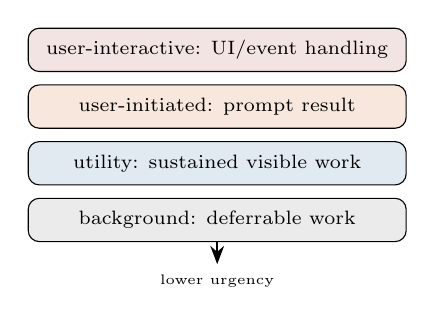
\begin{tikzpicture}[font=\scriptsize,>=Stealth,
        q/.style={draw,rounded corners,align=center,minimum width=4.8cm,minimum height=.55cm}]
        \node[q,fill=osred!13] (ui) at (0,2.5) {user-interactive: UI/event handling};
        \node[q,fill=osorange!16] (init) at (0,1.78) {user-initiated: prompt result};
        \node[q,fill=osblue!13] (util) at (0,1.06) {utility: sustained visible work};
        \node[q,fill=black!8] (bg) at (0,.34) {background: deferrable work};
        \draw[->,thick] (bg.south)--++(0,-.28)
          node[below,font=\tiny]{lower urgency};
      \end{tikzpicture}
      \vspace{.35em}
      \begin{lstlisting}
let q = DispatchQueue(label: "indexer",
                      qos: .utility)
q.async { rebuildSearchIndex() }
      \end{lstlisting}
  \end{columns}
  \begin{tcolorbox}[title=Interpretation,colback=osorange!5,colframe=osorange!70]
    QoS communicates intent to system frameworks and influences scheduling and resource policy; it is not a fixed CPU share or a hard deadline guarantee. Higher-priority work can also consume more energy.
  \end{tcolorbox}
  \note{Apple's QoS categories describe relative importance, and the system can use them to make CPU, I/O, and timer-latency trade-offs. The example uses utility for a long-running task the user is not actively waiting on. Use background for genuinely deferrable maintenance. Avoid making all work user-interactive: priority inflation harms responsiveness and energy efficiency elsewhere.}
\end{frame}

\begin{frame}{Cross-platform lesson: policy is not a deadline contract}
  \scriptsize
  \begin{tabularx}{\textwidth}{@{}lYYY@{}}
    \toprule
    \textbf{System} & \textbf{Application-facing control} & \textbf{What it helps express} & \textbf{What it does not prove} \\
    \midrule
    Linux & scheduler policy, nice, affinity, cgroups & class, relative share, placement/resource limits & end-to-end completion by an app deadline \\
    Windows & process class and thread-relative priority & relative urgency and interactive responsiveness & bounded response under arbitrary load \\
    Android & framework-managed threads and per-thread priority & UI/render urgency versus deferrable app work & stable frame timing across devices and thermal states \\
    macOS & QoS on dispatch queues and tasks & importance, latency/throughput, and energy intent & reserved CPU capacity or hard real-time behavior \\
    \bottomrule
  \end{tabularx}
  \vspace{.5em}
  \begin{block}{Engineering workflow}
    State the latency target, bound the work, avoid blocking critical paths, measure tail latency under contention, and define overload behavior before tuning priority.
  \end{block}
  \smallnote{Names and implementation details are release- and platform-dependent. Treat developer-facing priorities as policy inputs, not portable timing guarantees.}
  \note{This comparison distinguishes scheduling mechanisms from end-to-end guarantees. Android and macOS APIs classify or reprioritize work, but the complete path also includes framework queues, GPU/compositor or I/O work, power management, and contention. On Linux, cgroups can constrain groups of tasks, but a resource bound alone does not establish an application's deadline response time.}
\end{frame}

\begin{frame}{Priority inversion: a scheduling failure mediated by locks}
  \small
  \begin{center}
    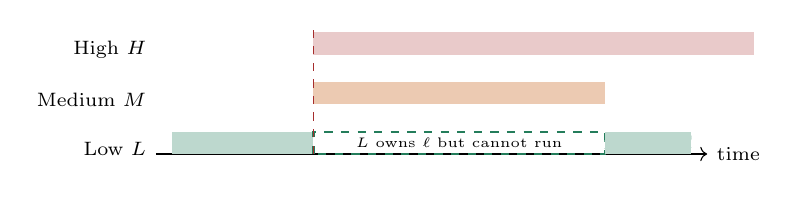
\begin{tikzpicture}[x=1cm,y=.63cm,font=\scriptsize]
      \draw[->] (0,0)--(7,0) node[right]{time};
      \node[anchor=east] at (0,2.1) {High $H$};
      \node[anchor=east] at (0,1.1) {Medium $M$};
      \node[anchor=east] at (0,.1) {Low $L$};
      \fill[osgreen!30] (.2,0) rectangle (2,.45) node[midway]{holds lock $\ell$};
      \fill[osred!25] (2,2) rectangle (6.8,2.45) node[midway]{blocked on $\ell$};
      \fill[osorange!35] (2,1) rectangle (5.7,1.45) node[midway]{preempts $L$};
      \draw[osgreen,dashed,thick] (2,0) rectangle (5.7,.45);
      \node[font=\tiny] at (3.85,.22){$L$ owns $\ell$ but cannot run};
      \fill[osgreen!30] (5.7,0) rectangle (6.8,.45) node[midway]{releases $\ell$};
      \fill[osred!25] (6.8,2) rectangle (7.6,2.45) node[midway]{runs};
      \draw[osred,dashed] (2,0)--(2,2.5);
    \end{tikzpicture}
  \end{center}
  A low-priority lock holder can indirectly delay a high-priority task while medium-priority work preempts the holder.
  \begin{itemize}
    \item \textbf{Priority inheritance:} temporarily raise the holder's priority until it releases the resource.
    \item \textbf{Priority ceiling:} protocol-specific ceiling rules bound blocking and prevent certain deadlocks.
    \item Neither protocol removes the need to bound critical-section duration and nested locking.
  \end{itemize}
  \note{Distinguish priority inversion from deadlock: in inversion, the holder can still run and release the lock, but interference delays it. The Mars Pathfinder incident is a classic historical illustration, not a proof that every inversion is catastrophic.}
\end{frame}

% Hands-on material is replaced below with safer, per-thread observations.
\iffalse
% Hands-on
\begin{frame}[fragile,allowframebreaks]{Hands-on Linux: Observe Scheduler Behavior}
  \small
  \textbf{Explore Linux Process and Scheduler States:}
  \begin{itemize}
    \item Open a terminal and use these commands to observe processes and their scheduling attributes.
    \item Pay attention to `PR' (priority), `NI' (nice value), `STAT' (process state), `%CPU'.
  \end{itemize}
  \vspace{0.3cm}
    \begin{lstlisting}[language=bash]
    # Show processes in a tree structure, including NI (nice) values
    htop --tree # or `top' and look at NI column
    
    # List processes with specific scheduling information
    # PID: process ID, COMM: command, NI: nice value, PRI: kernel priority
    # PCPU: CPU usage (percentage), STAT: process status
    ps -eo pid,comm,ni,pri,pcpu,stat --sort=-pcpu
    
    # Check real-time scheduling policy for a specific process (replace <pid>)
    # (e.g., `chrt -p <pid of your shell>')
    chrt -p <pid>
    
    # Run a process with a custom nice value (e.g., lower priority by setting nice 10)
    # This process will receive less CPU time from CFS.
    nice -n 10 dd if=/dev/zero of=/dev/null &
    
    # Run a process with a higher priority (negative nice value requires sudo)
    # (e.g., `sudo nice -n -10 dd if=/dev/zero of=/dev/null &')
    \end{lstlisting}

\framebreak
\vspace{0.3cm}
\textbf{Advanced: Inspecting Scheduler Debug Information (Requires root):}
\begin{itemize}
    \item This file provides detailed, low-level insights into the CFS scheduler's current state, including `vruntime' values.
\end{itemize}
\begin{lstlisting}[language=bash]
sudo cat /proc/sched_debug | less
\end{lstlisting}
\textit{(Look for sections like `runnable tasks' and their `vruntime' values.)}
\end{frame}

\fi

\begin{frame}[fragile]{Hands-on Linux: inspect scheduler behavior}
  \small
  \begin{itemize}
    \item Inspect per-thread policy, priority, nice value, state, and last CPU.
    \item Compare nice weights only under comparable fair-class workloads; affinity, cgroups, quotas, and other runnable work affect measured shares.
  \end{itemize}
  \begin{lstlisting}[language=bash]
# Per-thread view (Linux procps)
ps -eLo pid,tid,cls,rtprio,pri,ni,psr,stat,comm

# Inspect policy/parameters for one process or thread
chrt -p "$PID"

# Short-lived CPU-bound comparison; stop both jobs afterward
yes >/dev/null & a=$!
nice -n 10 yes >/dev/null & b=$!
sleep 5
ps -p "$a,$b" -o pid,ni,cls,pri,pcpu,comm
kill "$a" "$b"
wait "$a" "$b" 2>/dev/null
  \end{lstlisting}
  \smallnote{Optional, if installed/permitted: use \code{perf sched record} and \code{perf sched timehist} to inspect scheduling delays. Kernel debug interfaces vary by configuration and version.}
  \note{This is an observation exercise, not a precise share measurement. Positive nice lowers a task's fair-class weight. The shell starts two background jobs; kill and wait for them before leaving the exercise.}
\end{frame}

\section*{Summary}

% Summary
\begin{frame}{Key Takeaways}
  \scriptsize
  \begin{itemize}
    \item Deadline claims require a workload/platform model and analysis; a scheduler label alone is not a guarantee.
    \item RMS is fixed-priority: its Liu--Layland utilization test is sufficient, while response-time analysis can certify additional task sets.
    \item EDF's $U\leq1$ test is exact for ideal implicit-deadline uniprocessor tasks; constrained deadlines require demand analysis.
    \item Linux fair scheduling evolved from CFS accounting toward EEVDF; policy, per-CPU placement, and cgroups matter.
    \item Windows dispatches threads by priority; dynamic boosts are conditional and version/API context matters.
    \item Android frame pacing and macOS QoS both require matching work importance to the user-visible latency and energy goal.
    \item Blocking, overload, multicore interference, and WCET uncertainty often dominate the scheduler choice.
  \end{itemize}

  \begin{tcolorbox}[title=\textbf{Reflection Prompt: The Scheduler's Dilemma}, colback=blue!5!white, colframe=blue!75!black, fonttitle=\bfseries]
  For low-latency audio sharing a multicore phone with a CPU-heavy upload, specify the workload model, interference budget, admission policy, and fallback behavior before choosing a scheduler.
  \end{tcolorbox}
\end{frame}

% Next Week
\begin{frame}{Next Week Preview: Threads and Multithreading Models}
  \small
  \textbf{From Processes to Threads: Finer-Grained Concurrency}
  \begin{itemize}
    \item \textbf{Introduction to Threads:} Why threads are needed, process vs. thread.
    \item \textbf{User-Level vs. Kernel-Level Threads:} Understanding their differences and implementation.
    \item \textbf{Multithreading Models:} One-to-One, Many-to-One, Many-to-Many models.
    \item \textbf{Thread Libraries (`pthreads'):} How developers create and manage threads.
    \item \textbf{Thread Context Switching:} How it differs from process context switching.
  \end{itemize}
  \vspace{0.3cm}
  \pause
  \begin{tcolorbox}[title=\textbf{Prep Tip for Next Session}, colback=green!5!white, colframe=green!75!black, fonttitle=\bfseries]
  Review the concept of a process Control Block (PCB) and process context. Think about what information would still be unique to a thread and what could be shared among threads within the same process.
  \end{tcolorbox}
\end{frame}


\appendix
% Appendix numbering is enabled; appendix frames follow without a separate TOC entry.

% Quiz
\begin{frame}[allowframebreaks]{Quick Quiz: Real-Time \& Modern Scheduling}
  \small
  \textbf{Test Your Conceptual Understanding:}

  \vspace{0.3cm}

  \begin{enumerate}
      \item \textbf{Scenario:} Two implicit-deadline periodic tasks: A $(C=2,T=5)$ and B $(C=1,T=3)$.
      \begin{itemize}
          \item Which task has higher RMS priority? Compute $U$ and compare with the $n=2$ bound.
          \item What does the implicit-deadline EDF test conclude? Which result is sufficient versus exact?
      \end{itemize}
      \vspace{0.2cm}
      \item \textbf{True/False:} Two continuously runnable fair-class threads with nice 0 and nice +10 receive equal CPU shares on one otherwise idle CPU. State your assumptions.
      \vspace{0.2cm}
      \item \textbf{Define:} What is a temporary Windows dynamic-priority boost intended to improve, and why is it not a hard real-time guarantee?
      \vspace{0.2cm}
      \item \textbf{Application:} When is uniprocessor EDF utilization analysis insufficient for a multicore or constrained-deadline workload?
  \end{enumerate}

  \vspace{0.5cm}
  % \pause
  \begin{tcolorbox}[title=\textbf{Think \& Discuss}, colback=orange!5!white, colframe=orange!75!black, fonttitle=\bfseries]
  Formulate your answers before reviewing the solutions or discussing with peers.
  \end{tcolorbox}
\end{frame}

% Exercise
\begin{frame}[allowframebreaks]{Exercise: Real-Time Schedulability Analysis}
  \small
  \textbf{Part 1: RMS Schedulability Check}

  \textbf{Tasks:} (Execution Time $C_i$, Period $T_i$)
  \begin{itemize}
      \item Task A: $C_A=2$, $T_A=5$
      \item Task B: $C_B=1$, $T_B=4$
      \item Task C: $C_C=1$, $T_C=10$
  \end{itemize}
  \textbf{Task:}
  \begin{enumerate}
      \item Calculate the total CPU utilization ($U$) for this set of tasks.
      \item Calculate the RMS schedulability bound for $n=3$ tasks.
      \item Based on the RMS schedulability test, can these tasks be guaranteed to be scheduled by RMS? Show your calculations.
      \item What are the RMS priorities for Task A, B, and C?
  \end{enumerate}

  \vspace{0.5cm}
  % \pause

  \textbf{Part 2: Conceptual Comparison}

  \textbf{Scenario:} A new game console OS needs to be designed. It handles high-priority game rendering processes, background downloads, and occasional real-time voice chat.

  \textbf{Task:}
  \begin{enumerate}
      \item Would a pure FCFS scheduler be suitable? Why or why not?
      \item Would a pure EDF scheduler be a good choice for *all* tasks? Discuss potential benefits and drawbacks in this mixed environment.
      \item Propose a hybrid scheduling approach (e.g., using concepts from MLQ, Priority, and fairness) that could effectively manage these diverse workloads. Justify your proposal.
  \end{enumerate}

  \vspace{0.5cm}
  % \pause
  \begin{tcolorbox}[title=\textbf{Reminder}, colback=green!5!white, colframe=green!75!black, fonttitle=\bfseries]
  Remember to clearly state your assumptions and show all steps for calculations.
  \end{tcolorbox}
\end{frame}

% Appendix: Advanced Topics
\begin{frame}[allowframebreaks]{Advanced Topics to Explore}
  \small
  \textbf{Delving Deeper into Real-Time and Advanced Schedulers}

  \vspace{0.3cm}
  \begin{tcolorbox}[title=\textbf{I. Real-Time Scheduling Extensions}, colback=teal!5!white, colframe=teal!75!black, fonttitle=\bfseries]
  \begin{itemize}
      \item \textbf{Resource Sharing in RTOS:} Understanding solutions like Priority Inheritance Protocol (PIP) and Priority Ceiling Protocol (PCP) to prevent priority inversion.
      \item \textbf{Demand and response-time analysis:} dbf tests for EDF, response-time analysis with blocking and release jitter for fixed priority.
      \item \textbf{Aperiodic service:} deferrable/sporadic servers and reservation-based bandwidth isolation.
      \item \textbf{Multicore and mixed criticality:} partitioning, global scheduling, migration costs, and mode-change analysis.
  \end{itemize}
  \end{tcolorbox}

  \vspace{0.3cm}
  \begin{tcolorbox}[title=\textbf{II. Advanced Aspects of General-Purpose Schedulers}, colback=orange!5!white, colframe=orange!75!black, fonttitle=\bfseries]
  \begin{itemize}
      \item \textbf{Linux fair scheduling:} EEVDF eligibility/virtual deadlines, cgroup CPU weights and quotas, per-CPU run queues, and load balancing.
      \item \textbf{Windows:} base/dynamic priority, boosts, processor affinity, and processor groups (details depend on Windows release and API).
      \item \textbf{Scheduling interfaces:} compare Linux \code{sched_setscheduler}/\code{sched_setattr}/\code{setpriority} with Windows \code{SetThreadPriority}; inspect privilege and admission constraints.
  \end{itemize}
  \end{tcolorbox}

  \vspace{0.3cm}
  \begin{tcolorbox}[title=\textbf{III. Emerging \& Specialized Scheduling Areas}, colback=purple!5!white, colframe=purple!75!black, fonttitle=\bfseries]
  \begin{itemize}
      \item \textbf{Energy and heterogeneous CPUs:} DVFS, capacity-aware placement, thermal constraints, and big.LITTLE scheduling.
      \item \textbf{Virtualization and nested scheduling:} how guest vCPUs compete with host tasks and how steal time affects deadlines.
      \item \textbf{Alternative policies:} lottery/stride proportional share, gang scheduling, GPU scheduling, and network packet schedulers.
  \end{itemize}
  \end{tcolorbox}
\end{frame}

\begin{frame}{Primary references and version notes}
  \scriptsize
  \begin{itemize}
    \item Linux kernel, \emph{EEVDF Scheduler}: \url{https://docs.kernel.org/scheduler/sched-eevdf.html}
    \item Linux kernel, \emph{CFS Scheduler}: \url{https://docs.kernel.org/scheduler/sched-design-CFS.html}
    \item Linux man-pages, \emph{sched(7)} scheduling policies: \url{https://man7.org/linux/man-pages/man7/sched.7.html}
    \item Linux kernel, \emph{Deadline Task Scheduling}: \url{https://docs.kernel.org/scheduler/sched-deadline.html}
    \item Microsoft Learn, \emph{Scheduling Priorities}: \url{https://learn.microsoft.com/en-us/windows/win32/procthread/scheduling-priorities}
    \item Microsoft Learn, \emph{Priority Boosts}: \url{https://learn.microsoft.com/en-us/windows/win32/procthread/priority-boosts}
    \item Android Developers, \emph{Better performance through threading}: \url{https://developer.android.com/topic/performance/threads}
    \item Android Developers, \emph{Process.setThreadPriority}: \url{https://developer.android.com/reference/android/os/Process}
    \item Apple Developer, \emph{DispatchQoS}: \url{https://developer.apple.com/documentation/dispatch/dispatchqos}
    \item C. L. Liu and J. W. Layland, “Scheduling Algorithms for Multiprogramming in a Hard-Real-Time Environment,” \emph{JACM}, 20(1), 1973, pp. 46--61.
  \end{itemize}
  \begin{tcolorbox}[title=Version discipline,colback=blue!5,colframe=blue!65]
    Scheduler internals and platform APIs change. CFS is retained as a historical/accounting model; consult target Linux, Android, Windows, and macOS documentation before making implementation-specific claims.
  \end{tcolorbox}
\end{frame}

\end{document}

